\section{Analysis strategy}
\label{sec:db:strategy}

This analysis is a completely general search for a particle with unknown mass, \mass\db, and
lifetime, \lifetime\db.
Exhaustive details of the analysis strategy can be found in \Ref{Williams:2015xfa}, but the
following section will outline the important points.
Broadly, the search involves a frequentist scan of the dimuon invariant mass spectrum,
separated into two bins in decay time, from
\btokstrmumu for an excess of events consistent with \dbtomumu.
Firstly, an explanation of the search in the mass dimension will be presented, and then extended to
to deal with the decay time dimension.


\subsection{Searching in the mass dimension}
A scan in mass is performed where the test mass, \mass{t}, is incremented in steps of
$\tfrac12\sigmam$, where $\sigmam$ is the local mass resolution defined at \mass{t}.
In this analysis, \sigmam lies in the range $1\lesssim\sigmam\lesssim6\mev$.
At each \mass{t} a signal region is defined as $|m-\mass{t}|<2\sigmam$ and a sideband, or
background, region is defined as $3\sigmam<|m-\mass{t}|<(2x+3)\sigmam$, where
$x$ defines the width of the sideband regions with respect to the signal region.
The purpose of constructing the two regions is to use the sideband regions to estimate the background
contribution in the signal window.

At each mass point in the search the number of events in the signal region, $n_s$, and the number
of events in the background events, $n_b$, are counted.
If the background is, on average, linear in the local mass region, and if there is no signal
contribution: $\langle n_s\rangle=\tfrac12\langle n_b\rangle$.
However, if there is evidence of signal, then $n_s=s+b$, where $s$ is the
number of signal events, and $b$ is the background component in the signal region which is
estimated from the sideband regions.
Thus, one can construct a likelihood:
\begin{equation}
  \mathcal{L}(n_s, n_b | s, b) =
  \mathcal{P}(n_s, s+b) \cdot
  \mathcal{P}(n_b, xb),
  \label{eq:db:like1}
\end{equation}
where $\mathcal{P}(n, \lambda)$ is the probability of observing $n$ from a Poisson distribution
parameterized by $\lambda$.
This is simply the likelihood of the background estimate from the sidebands fluctuating to
the observed number of events in the signal region.
%Twice, so far, the local linearity of the background has been mentioned as the sole assumption,
%this is important to bare in mind throughout.
%The sole assumption is that the background is locally-linear at all values of \mass{t}.

The likelihood given in \Eq{eq:db:like1} assumes that the background is, on average, exactly
linear, and therefore that the size of the sideband region is always factor of $x$ larger than the
signal region.
%But, this may not be the case.
In reality, the sideband region is a not precisely a factor $x$ larger than the signal region, but
rather some factor $y$.
The uncertainty between $x$ and $y$, called $\sigma_y$,
is chosen depending on \mass{t}, and
accounted for in the likelihood directly, by
modifying the likelihood function to be
%The problem with \Eq{eq:db:like1} is that, while $x$ has been chosen, deviations from a linear
%background distribution mean that the actual sideband size with respect to the signal region is
%not, in fact, $x$.
%Rather, the actual scale factor is some $y$, with some uncertainty $\sigma_y$.
%This can be accounted for by including an additional term in the likelihood
\begin{equation}
  \mathcal{L}(n_s, n_b, x | s, b, y) =
  \mathcal{P}(n_s, s+b) \cdot
  \mathcal{P}(n_b, yb) \cdot
  \mathcal{G}(y,x,\sigma_y).
  \label{eq:db:like2}
\end{equation}
Here, $\mathcal{G}(n, \mu, \sigma)$ is the probability of observing $n$ given a Gaussian
distribution with a mean, $\mu$, and standard deviation, $\sigma$.
This modification allows the uncertainty on the background shape to be immediately accounted for in
the method, meaning that no additional systematic uncertainty needs to be added.

In the absence of resonances,
the dimuon background from the \sm decay \btokstrmumu is expected to be locally-linear
to less than $1\pc$ over the entire mass range.
However, then inclusion of resonances can lead to significant departures from linearity, dependent
upon the resonance's width ($\Gamma$), magnitude, and the value of $x$.
Table~\ref{tab:db:bkg} lists a number of mesons, $X$, that decay to a dimuon final state and could
contribute as background to the decay \decay{\Bd}{\Kstarz\mumu}.
Wide resonances, $\Gamma\gtrsim20\sigmam$, such as the $\rho$,
are sufficiently wide not as to be problematic even if
they dominate the local background distribution.
Conversely, narrow resonances where $\Gamma\lesssim5\sigmam$ lead to significant deviations from a
locally-linear background and must be vetoed.
Dimuon decays of the \phii, \jpsi, and \psitwos mesons have the highest branching fractions, and
are also among the
narrowest resonances; they are therefore vetoed.
Intermediate resonances, $5\lesssim\Gamma\lesssim20\sigmam$, are considered on a case-by-case
basis since they are only troublesome if they account for a large fraction of the local background.
For this analysis, these ranges roughly translate to requiring that resonances with $\Gamma<25\mev$
will be vetoed, and those with $\Gamma>125\mev$ shall be ignored.
Other resonances given in \Table{tab:db:bkg} are broad and contribute to the dimuon
structures at low mass.
It is shown in \Ref{Williams:2015xfa} that the local-linearity approximation is accurate to
\approx$5\pc$ in regions where there may be contributions from wide resonances.
Below the mass of the \jpsi the values of $x=5$ and $\sigma_y=0.05$ are chosen.

\begin{table}
  \caption[Total branching fractions for decays with the final state \btokstrmumu]
  {
    Selected particles properties for mesons which decay into a dimuon pair final state, and
    the branching
    fractions for the relevant decays~\protect\cite{PDG2014}.
    Central values of mass and width are given in MeV.
  }
  \label{tab:db:bkg}
  \begin{center}
      %\begin{tabular*}{\textwidth}{lrc @{\extracolsep{\fill}} r @{\extracolsep{\fill}} rc}\toprule
    \scalebox{0.9}{
      \begin{tabular*}{1.1\textwidth}{lrc @{\extracolsep{\fill}} r @{\extracolsep{\fill}} r
        @{\extracolsep{\fill}} c}
        \toprule
        \cellc{Meson ($X$)} & \cellc{Mass} & \cellc{Width}
        & \cellc{$\BF(\decay{\Bd}{\Kstarz X})$}
        & \cellc{$\BF(\decay{X}{\mumu})$}
        & \cellc{$\BF_\mathrm{tot}(\decay{\Bd}{\Kstarz\mumu})$}
        \\\midrule
        ${\eta}$        & $\pz547.9$ & $\pzz0.001$
        & $(1.59\pm0.10)\e{-5}$
        & $(5.8\pz\pm0.8\pz)\e{-6}$
        & $(9.2\pm1.4)\e{-11}$
        \\
        ${\rho}$   & $\pz775.3$ & $147.8\pzz$
        & $(3.9\pz\pm1.3\pz)\e{-6}$
        & $(4.55\pm0.28)\e{-5}$
        & $(1.8\pm0.6)\e{-10}$
        \\
        ${\omega}$ & $\pz782.7$ & $\pzz8.5\pzz$
        & $(2.0\pz\pm0.5\pz)\e{-6}$
        & $(9.0\pz\pm3.1\pz)\e{-5}$
        & $(1.8\pm0.8)\e{-10}$
        \\
        ${\phi}$  &   $1019.5$ & $\pzz4.3\pzz$
        & $(1.00\pm0.05)\e{-5}$
        & $(2.87\pm0.19)\e{-4}$
        & $(2.9\pm0.2)\e{-\pz9}$
        \\
        ${\Dz}$         &   $1864.8$ & $\pz10.1\pzz$
        & $(4.2\pz\pm0.6\pz)\e{-5}$
        & $<6.2\e{-9}$
        & \makebox[\widthof{$(2.9\pm0.2)\e{-\pz9}$}][r]{$<2.6\e{-14}$}
        \\
        \jpsi & $3096.9$ & $\pzz0.093$
        & $(5.96\pm0.03)\e{-2}$
        & $(1.32\pm0.06)\e{-3}$
        & $(7.9\pm0.4)\e{-\pz5}$
        \\
        \psitwos & $3686.1$ & $\pzz0.299$
        & $(7.9\pz\pm0.9\pz)\e{-3}$
        & $(6.0\pz\pm0.4\pz)\e{-4}$
        & $(4.7\pm0.6)\e{-\pz6}$
        \\
        \bottomrule
      \end{tabular*}
    }
  \end{center}
\end{table}

Resonances that have a natural width in the intermediate region, $5\lesssim\Gamma\lesssim20\sigmam$, are
various \ccbar states with masses above the mass of the \psitwos.
For example, there is contribution from the $\psi(4160)$ which was observed by \lhcb in the decay
\decay{\Bp}{\Kp\mumu}~\cite{LHCb-PAPER-2013-039}.
All known charmonium resonances in this region are wide,
$\Gamma\sim70\mev$, and are dealt with by reducing the size of the sidebands and increasing the
uncertainty on the background shape, by setting $x=1$ and $\sigma_y=0.1$.
%A summary of the values of $x$ and $\sigma_y$ for different regions of \mass{t} are given in
%\Table{tab:db:xsigmay}.


%\begin{table}
  %\caption[Values of $x$ and $\sigma_y$ used]
  %{
    %Values of $x$ and $\sigma_y$ used above and below the \jpsi mass.
  %}
  %\label{tab:db:xsigmay}
  %\begin{center}
    %\begin{tabular}{ccc}\toprule
      %Region & $x$ & $\sigma_y$ \\\midrule
      %$\mass{t}<\mass{\jpsi}$ & 5 & 0.05 \\
      %$\mass{t}>\mass{\jpsi}$ & 1 & 0.10 \\
      %\bottomrule
    %\end{tabular}
  %\end{center}
%\end{table}

Interference effects between
\btokstrmumu and \decay{\Bd}{\Kstarz\rho}, where \decay{\rho}{\mumu}, could lead to non-linearity
in the background shape, despite the fact that the total branching fractions of
$\decay{\Bd}{\Kstarz\rho(\to\mumu)}$ decay is so small that less than one event is expected in the
data sample.
However, this deviation can only be a maximum of \approx$5\pc$, which is already accounted for in
the choice of $\sigma_y=0.05$.

The contribution from the decay \decay{\phi}{\mumu} to the $\Kstarz\mumu$ final state is removed by
excluding dimuon candidates in the range $1000<\mass{\mumu}<1040\mev$.
Vetoed regions for the \jpsi and \psitwos are calculated using a theoretical
model which can account for the interference effects between the
\decay{\ccbar}{\mumu} resonances and the non-resonant \mumu component~\cite{Bobeth:2011nj}.
The model is used to generate \glspl{PDF} with different phase differences between the resonant and
non-resonant components, which is then convolved with a double Gaussian function to account for
detector resolution effects; these are shown in \Fig{fig:db:ccbar}.
%possible deviation from non-linearity in the dimuon spectrum.
%These \glspl{PDF} are shown in \Fig{fig:db:ccbar}.
%This model is used to model the shape of these two large \ccbar contributions to the \mumu final
%state with different phases between resonant and non-resonant components, and then this is
%convolved with a Gaussian to account for the resolution of the \lhcb detector, as shown in
%\Fig{fig:db:ccbar}.
After smearing, the \glspl{PDF} are then used to
calculate the regions around the \jpsi and \psitwos where the
background is locally linear to better than $5\pc$ for various values of $x$.
The resulting veto regions which are very similar to those used in
\Ref{LHCb-CONF-2015-002}, except that the upper boundary of the \psitwos veto is extended to cover
the $\psi(3770)$.
All the vetoed regions to remove narrow resonances decaying via \decay{X}{\mumu}, are summarized in
\Table{tab:db:narrow}.

\begin{figure}
  \begin{center}
    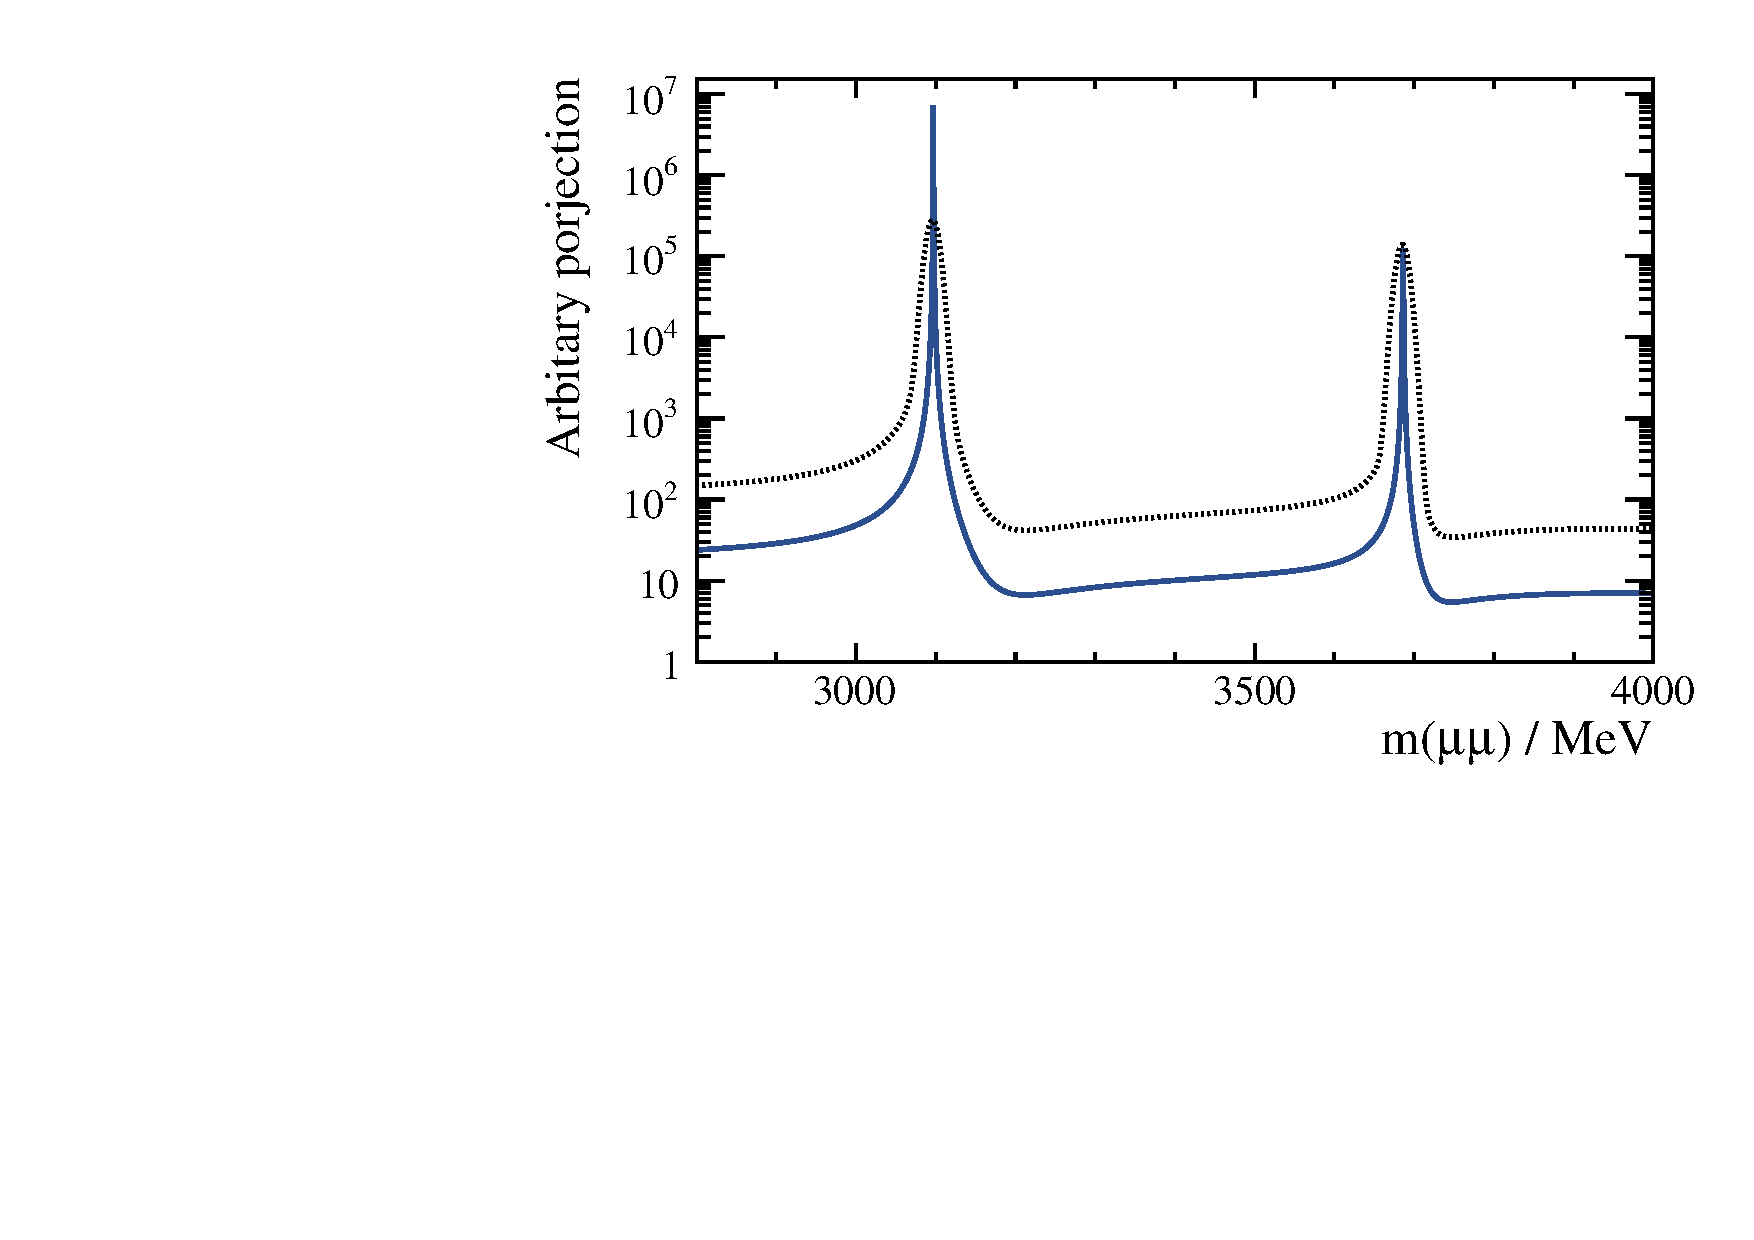
\includegraphics[width=0.48\textwidth]{ccbar_0_0}
    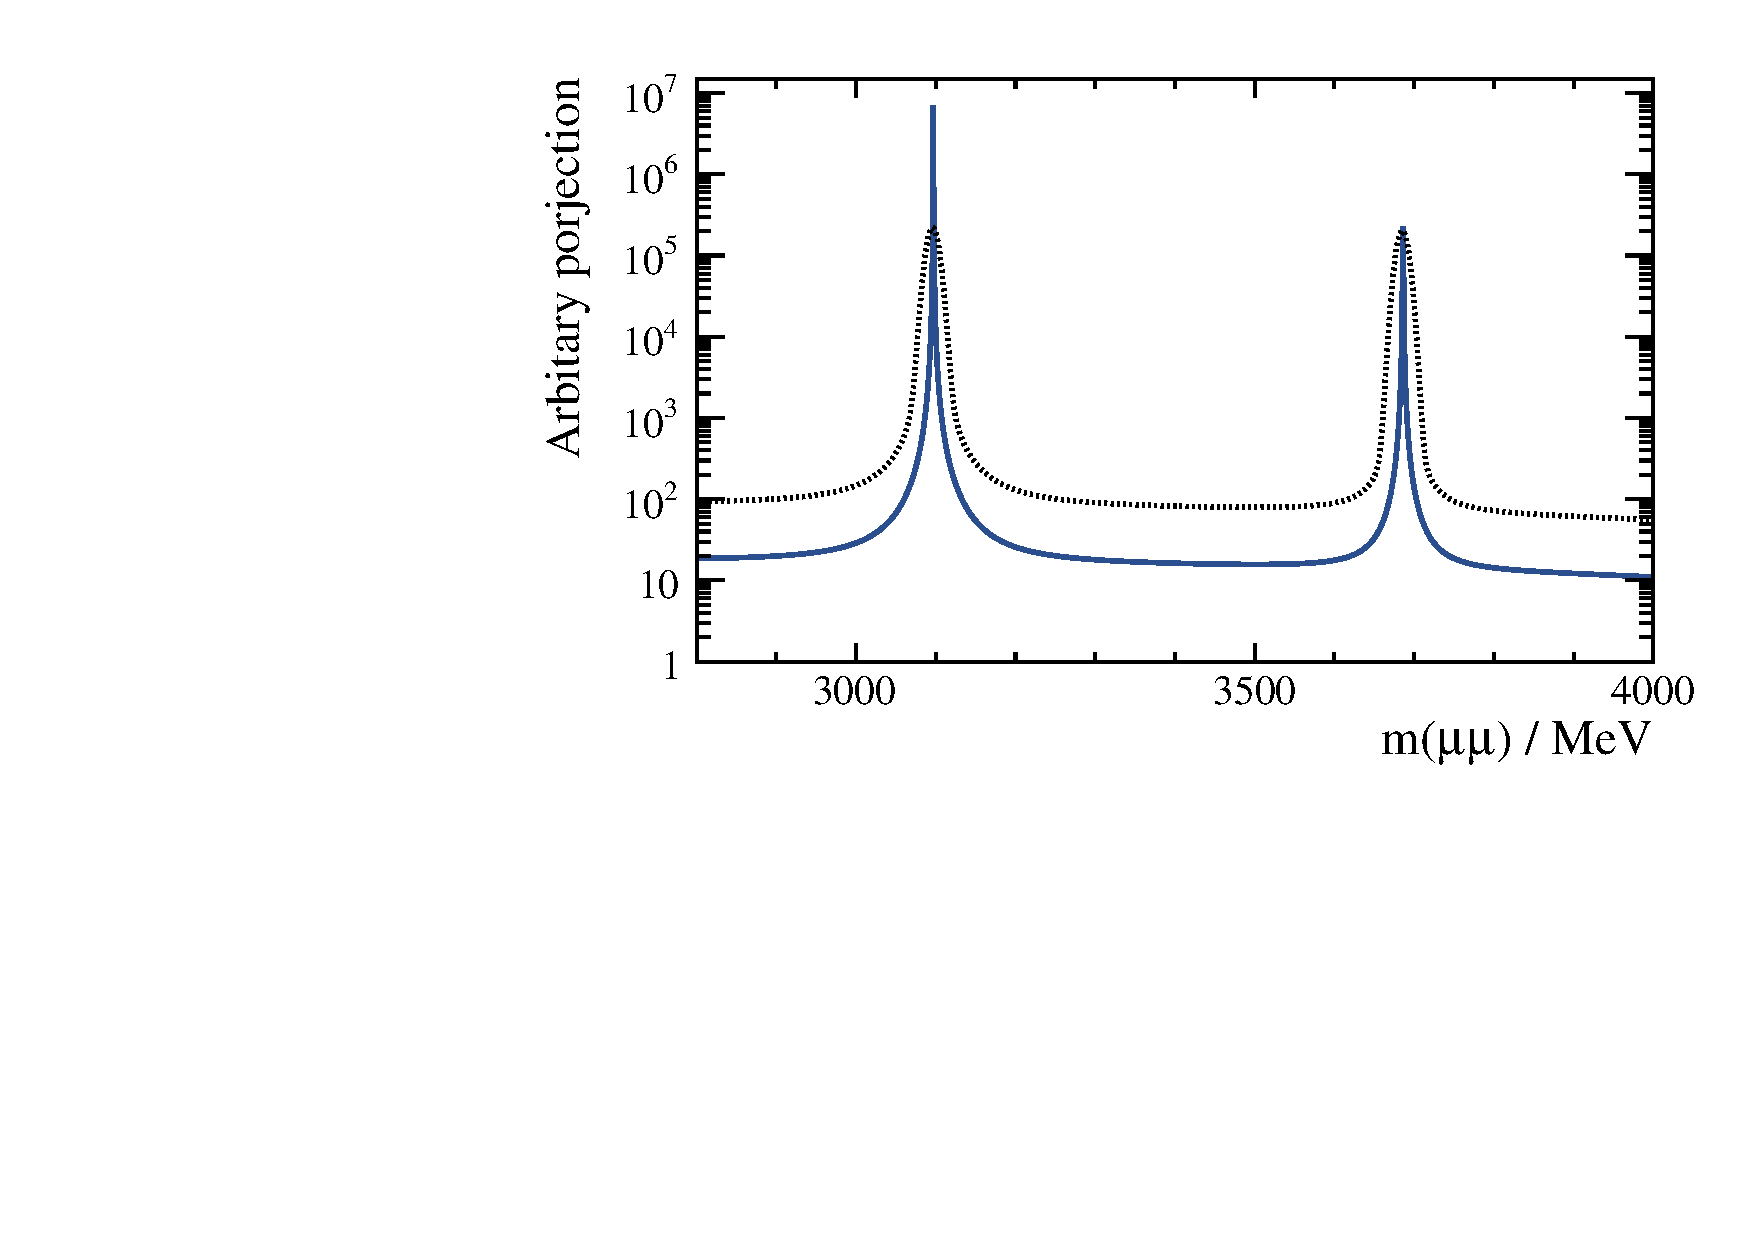
\includegraphics[width=0.48\textwidth]{ccbar_1_57_1_57}
    \caption[Theoretical distributions of \ccbar resonances interfering with a non-resonant
    coponent]
    {
      Theoretical distributions of the decays \jpsitomumu and \decay{\psitwos}{\mumu} interfering
      with a non-resonant dimuon component using a model in Ref.~\protect\ref{Bobeth:2011nj} with
      (left) no phase difference, and
      (right) maximal phase difference.
      The solid blue line shows the raw model, and the dotted line is the same distribution which
      has been convolved with a Gaussian to account for detector resolution effects.
    }
    \label{fig:db:ccbar}
  \end{center}
\end{figure}


\begin{table}
  \caption[Summary of veto regions for onia]
  {
    Summary of the vetoes regions in \mass{\mumu} to remove the contributions from the decays
    \decay{\phi}{\mumu} and various narrow \decay{\psi}{\mumu} to the dimuon distribution.
  }
  \label{tab:db:narrow}
  \begin{center}
    \begin{tabular}{lc}\toprule
      Resonance(s) & Vetoed region (MeV) \\\midrule
      \phii & $1000<\mass{\mumu}<1040$ \\
      \jpsi & $2960<\mass{\mumu}<3204$ \\
      \psitwos, $\psi(3770)$ & $3614<\mass{\mumu}<3875$ \\
      \bottomrule
    \end{tabular}
  \end{center}
\end{table}

%Narrow resonances, falling in the $\Gamma\lesssim5\sigmam$ region are removed:
%these include the \phii, \jpsi, and \psitwos.
%The decay \decay{\phi}{\mumu} is removed by excluding dimuon candidates in the range
%$1000<\mass{\mumu}<1040\mev$.
%Charmonuim resonances are vetoed using

%The largest deviations from a locally-linear background are at the $5\%$ level, which is
%natrually accounted for by setting \

%Practically, the resonances that must be removed from the background are the \phi, \jpsi, \psitwos

The profile likelihood, $\Lambda$, is defined as
\begin{equation}
  \Lambda(s|n_s,n_b) =
  \frac
  {\mathcal{L}(s, \hat{b}(s), \hat{y}(s) | n_s, n_b, x)}
  {\mathcal{L}(\hat{s}, \hat{b}, \hat{y} | n_s, n_b, x)},
  \label{eq:profilelike1}
\end{equation}
where $\hat{s}$, $\hat{b}$, and $\hat{y}$ are chosen to maximize the likelihood; the functions
$\hat{b}(s)$ and $\hat{y}(s)$ maximize the likelihood for a given $s$.
%The solutions to these functions can be calculated analytically, with few assumptions made,
%and thus the likelihood can be minimized with minimal computational power.
%The profile likelihood can then be formed in the same way as in \Eq{eq:profilelike1} and solved
%analytically.
The test statistic used for discovery is $\Lambda(0)$, where $\hat{s}$ is restricted to the
physical region, such that $\hat{s}\geq 0$.


\subsection{Searching in the lifetime dimension}
Sensitivity to the lifetime of the \db, \lifetime{\db}, is introduced by splitting the data at each
test mass into two regions: a prompt and a displaced region, defined by $\tau<3\sigmat$ and
$\tau>3\sigmat$ respectively; where \sigmat is defined to be the local decay time resolution.
The likelihood for each decay time bin is defined using \Eq{eq:db:like2}, and the joint likelihood is
simply the product of the two
individual likelihoods
\begin{align}
  \mathcal{L}(n^p_s, n^p_b, n^d_s, n^d_b, x | s^p, b^p, y^p, s^d, b^d, y^d) &=
  \mathcal{L}(n^p_s, n^p_b, x | s^p, b^p, y^p)\nonumber\\
  &\quad\times\mathcal{L}(n^d_s, n^d_b, x | s^d, b^d, y^d).
  \label{eq:db:liketau}
\end{align}
In these expressions the superscripts $p$ and $d$ denote the prompt and displaced regions,
respectively.

The information supplied by the addition of two bins in the lifetime dimension is approximately
optimal for all \db lifetimes, except for when $\tau\sim3\sigmat$.
In this case, it is marginally more optimal to include shape information of the background
distribution from the sidebands; but this introduces
significantly more complications to the analysis.
%and there is no reason to believe that the \db has
%a lifetime $\tau\sim3\sigmat$ \emph{a priori}.
Therefore background shape information is not used.


\subsection[Calculation of $p$-value]
{Calculation of $\boldsymbol{p}$-value}
At each \mass{t}, a $p$-value is calculated using the profile likelihood of the joint likelihood
given in \Eq{eq:db:liketau}.
Because there are $\mathcal{O}(1000)$ test masses, each of which is not completely independent the
look-elsewhere effect must be accounted for.
To do this the minimum local $p$-value is translated into a global $p$-value using a trials factor
which is calculated using an ensemble of toys.

%\bam{CLARIFY}
After the $p$-value at each \mass{t} is calculated, the region in which the lowest $p$-value
consistent with zero signal will be isolated and removed from the sample; leaving data which
which is entirely background.
This is assuming that there is only one \np particle that can be observed in this analysis.
The remaining background-like distribution is then turned into a \PDF\ --- where the region that is
removed is interpolated across --- from which toy datasets can be generated.
A conversion from local to global $p$-value can then be calculated by generating 10 million toy
datasets.


\subsection{Limits}
Upper limits will be set as a function of \mass{\db} and \lifetime{\db}.
This requires further modification to the likelihood function to account for the relationship
between the number of signal events in the prompt and displaced regions for a given value of
decay time.
An additional Gaussian terms are added: one to account for the uncertainty in the fraction of
signal events that are observed in the two lifetime regions, and another to account for the
uncertainty in the efficiency ratio with respect to the normalization channel.
The resulting likelihood for a given \mass{\db} and \lifetime{\db} is given by:
\begin{align}
  \like\big(n_s^p, n_b^p, n_s^d, n_b^d, x, \tau | \dots\big) &=
   \like\big(n_s^d, n_b^d, x | \varepsilon s f,b^p,y^p\big) \nonumber\\
   &\quad\times\like\big(n_s^p, n_b^p, x | \varepsilon s(1-f),b^d,y^d\big)\nonumber\\
   &\quad\times\mathcal{G}\big(f, \xbar{f}(\tau_\db),\sigma(f)\big)
   \times\mathcal{G}\big(\varepsilon, \xbar{\varepsilon}(\tau_\db),\sigma(\varepsilon)\big),
   \label{eq:db:lim}
\end{align}
where the fraction of signal events in the prompt region is given by $f$,
which has an expected value from simulation $\xbar{f}$ and an uncertainty $\sigma(f)$.
The same nomenclature is used for the efficiency measured relative to the normalization channel,
$\varepsilon$.

The normalization channel used will be the \sm decay \btokstrmumu, restricted to the region
$1.1<\qsq<6.0\gevgev$.
This range is chosen to minimize theoretical uncertainties at low and high \qsq and reduce
experimental uncertainties by removing the region around the \phii meson which has a central value
of mass in \qsq of \approx$1.04\gevgev$.














